
\section{Flapping Wing simulation}

An application example of \acrshort{precice}-\acrshort{mbdyn} coupling in the study of \acrshort{fsi} problems can be found in \cite{heathcote2008effect}, in which the effect of spanwise wing flexibility on thrust, lift and propulsive efficiency of a rectangular wing oscillating in pure heave is analyzed by means of water tunnel experiments.

The study shows that, for some oscillating frequencies, a degree of spanwise flexibility yields a small
increase in thrust coefficient and a small decrease in power-input requirement, resulting in higher overall efficiency.

\subsection{Experimental setup}

Before describing the \acrshort{fsi} model and the simulation, it is necessary to briefly introduce the experimental setup.

The study considers three types of rectangular wings, with profile \textit{naca 0012} and with different section properties, as shown in Figure~\ref{fig:profiles0012}. The section labeled (i) is considered \textit{inflexible}, the one labeled (ii) is considered \textit{flexible} and the last one \textit{highly flexible}.

\begin{figure}[htbp!]
	\centering
	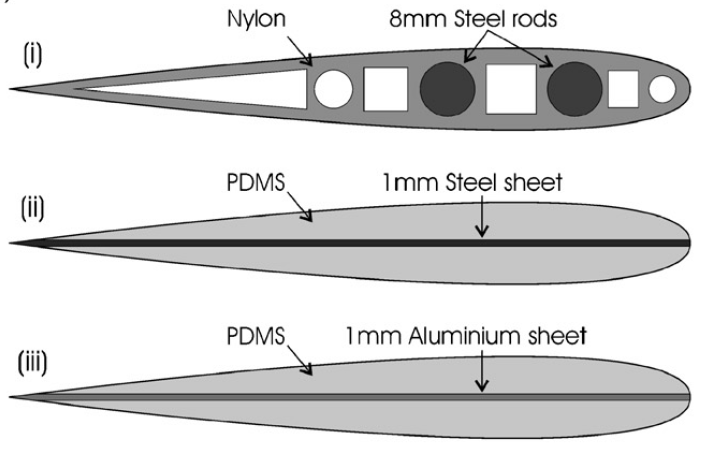
\includegraphics[width=0.7\textwidth]{images/profiles0012}
	\caption{wing section properties (image taken from \cite{heathcote2008effect})}
	\label{fig:profiles0012}
\end{figure}

Each wing has the following dimensions: $100$\si{mm} chord and $300$\si{mm} span.

The experimental setup is shown in Figure~\ref{fig:0012exp}. The displacement of the root section is given by $s = a_{ROOT} \cos(\omega t)$, where $a_{ROOT} = 0.175c$. The flow velocity $U_0$ is in the range $1-3$\si{m.s^{-1}}. The following dimensionless parameters are considered:

\begin{itemize}
	\item $Re = \frac{\rho U_0 c}{\mu}$: Reynolds number
	\item $k_G = \frac{\pi f c}{U_0}$: Garrick reduced frequency
	\item $S_r = \frac{2f a_{MID}}{U_0}$: Strouhal number at mid-span
\end{itemize}

\begin{figure}[htbp!]
	\centering
	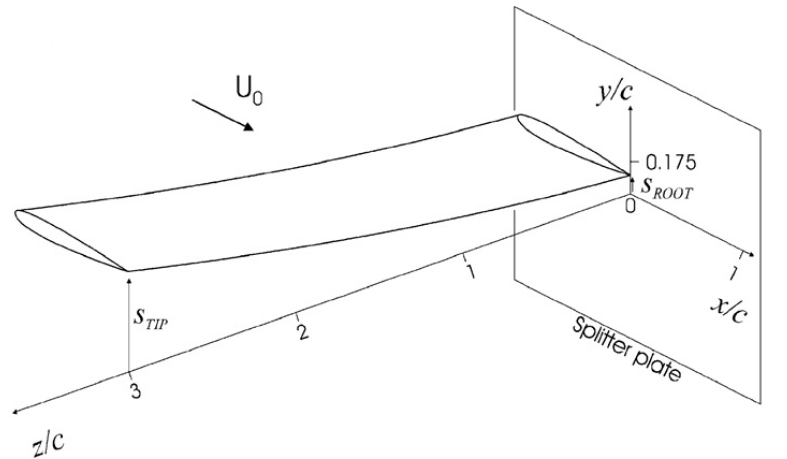
\includegraphics[width=0.7\textwidth]{images/naca0012_exp}
	\caption{experimental setup (image taken from \cite{heathcote2008effect})}
	\label{fig:0012exp}
\end{figure}

Experiments are carried out for the three types of wings in the following ranges: $Re=1\cdot10^4-3\cdot10^4$ and $k_G=0-7$.

The results give information concerning the average thrust coefficient $C_T = \frac{T}{\frac{1}{2}\rho U_0^2c}$ over a finite number of cycles and the mean power input coefficient $\bar{C}_P = \frac{\bar{F_y v}}{\frac{1}{2}\rho U_0^3c}$.

Besides, information concerning the ratio $\frac{a_{TIP}}{a_{ROOT}}$ and tip phase lag $\phi$ are given.

\subsection{Simulation setup}







